\subsection{Punching shear}
Early foundations for punching shear design was laid in \cite{talbot1913reinforced} though through examination was not carried out until much later \citep{elstner1956shearing,moe1961} without moment application that are reviewed in detail by \cite{ghoreishi2013review,yang2011data,hamada2008evaluation}. 
\begin{figure}\centering
    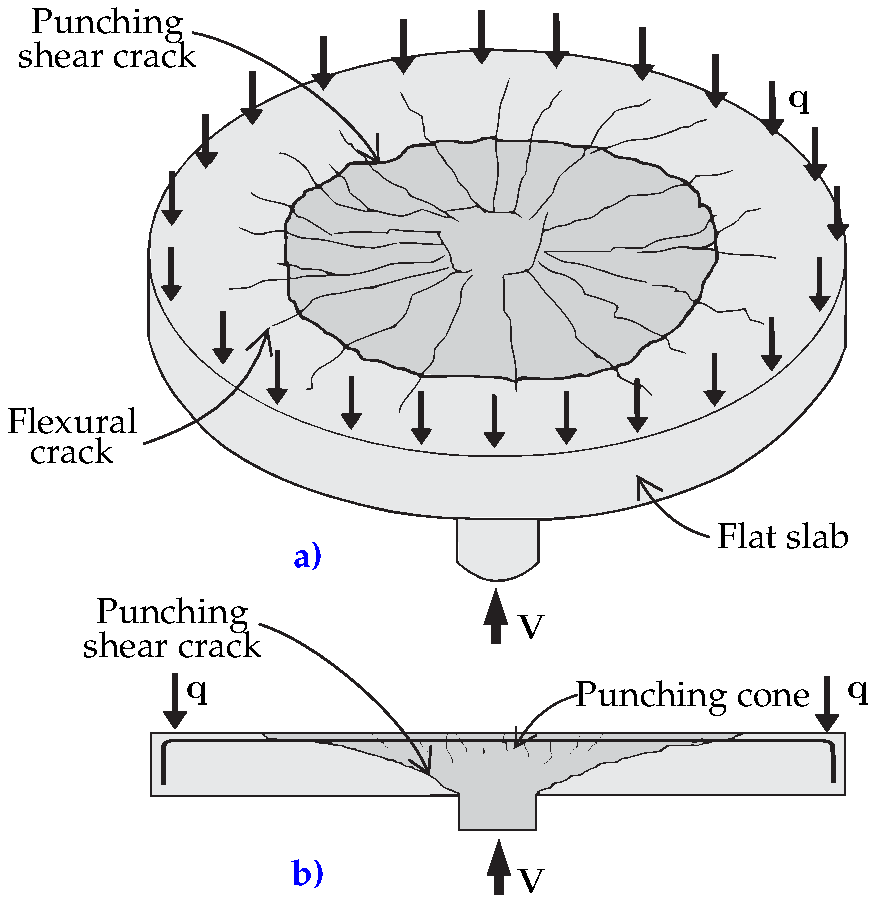
\includegraphics[width=\columnwidth]{Figures/tikzout/b16if1.pdf}\caption{Isolated interior flat slab-column connection region and typical punching shear failure surface, adapted from \cite{bompa2016b}: a) Isometric view; b) Section view.}\label{b16if1}
    \end{figure}
On the other hand \cite{kinnunen1960} proposed that flat slab punching strength is related to slab flexural deformations in the column vicinity that was further improved by \cite{shehata1989punching,broms1990}.

Concrete strength, longitudinal reinforcement ratio and slab thickness have been accounted as main influential factors for punching shear performance of slab column connections\citep{yitzhaki1966,regan1981,tian2008behavior,marzouk1991} that are considered in punching shear capacity estimation calculations in various national codes\citep{gb500102010,aci31819,bs81101997,en1992}.


Column connection region behavior in reinforced concrete elements is characterized by flexural crack developments at incipient loading stages (\ref{b16if1}a and \ref{b16if2}c). 

Typically with low reinforcement ratios at an ultimate state these cracks may govern connection behavior leading to a potential yield of longitudinal reinforcement (\ref{b16if3}c) \citep{hallgren1996punching}.  If flexural behavior doesn't govern and with reinforcement stresses nigh on bar yield stress, flexural cracks would propagate into shear cracks leading to a failure mode defined as flexural punching\citep{fib2001}.

    \begin{figure}\centering
        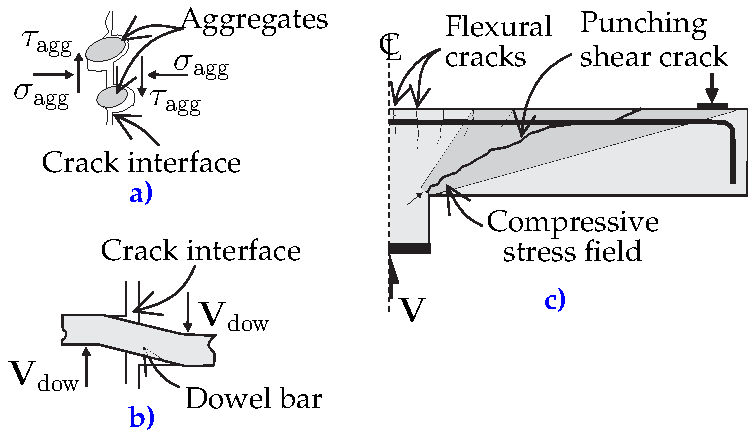
\includegraphics[width=\columnwidth]{Figures/tikzout/b16if2.pdf}\caption{Slab-column connection cracks, adapted from \cite{bompa2016b}: a) Aggregate interlock; b) Dowel action; c) Compression field.}\label{b16if2}
        \end{figure}

In case of high reinforcement ratios the slab behaves stiffer with reinforcements bearing lower stresses and higher stresses concentrated in the inclined concrete compression zone developed near the column (\ref{b16if3}a)\citep{hallgren1996punching}. Punching shear failure is described as the development of a diagonal crack with variable inclination starting from the column face on the slab compression side and ending at the slab tension face resulting in the dislocation of a conical body of concrete slab (\ref{b16if1}) \citep{regan1986}.


\begin{figure}\centering
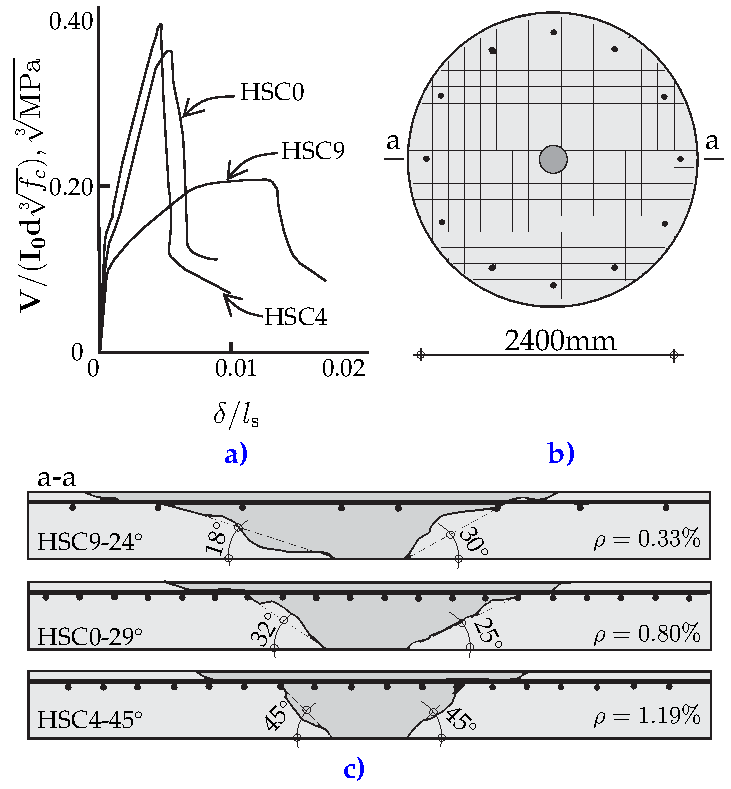
\includegraphics[width=\columnwidth]{Figures/tikzout/b16if3.pdf}\caption{Test results (HSC0, HSC4, HSC9) carried out by \cite{hallgren1996punching},  adapted from \cite{bompa2016b}: a) Structural response; b) In-plane geometrical configuration; c) Sectional view of saw cuts.}\label{b16if3}
\end{figure}
\begin{figure}\centering
    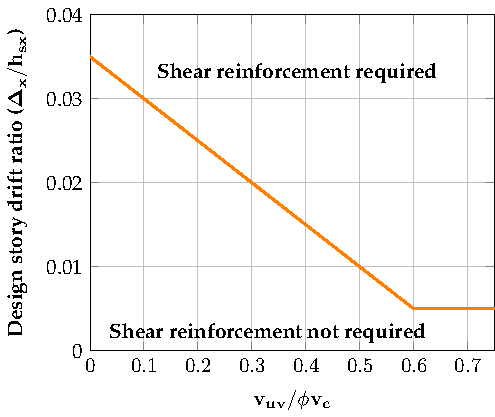
\includegraphics[width=\columnwidth]{Figures/tikzout/fr181451.pdf}\caption{Slab shear reinforcement requirement criteria, recreated from \cite{aci31819}.}\label{fr181451}
    \end{figure}
Typically in concrete members shear is carried by \begin{itemize}\item the interlock and frictional resistance of the cracked interface aggregates against crack slip and growth\citep{walraven1981}, \item dowel bar shearing\citep{dei1987,dei1992,ince2007,paulay1974,taylor1970}, \item transmission through the concrete section compression zone\citep{chana1987}, \item and residual stress transfer through the crack tip(\ref{b16if2} a,b)
\end{itemize}
Stress distribution in the column-slab connection region governs punching shear crack inclination angle and the slab punching shear strength is governed by the amount of shear carried or resisted by the cracked interface. The inclination angle and punching shear capacity depend on member geometry\footnote{Depth, slenderness, column dimensions to slab thickness ratio.} and structural parameters\footnote{Material strengths, aggregate properties, reinforcement layout and so on.}. As the inclination angle reduces and the cracked interface parallels the slab faces further, the interlocking surface widens, also more bars get involved in dowel action thus larger amounts of shear are transferred. 


\cite{zheng2023} Carried out a thorough nonlinear finite element study verified based on 14 test results out of the literature and simulating 49 slab-column connections evaluating shear span ratio and slab aspect ratio effects.

\cite{tomas1993} investigated the punching shear behavior of normal weight and light weight concrete slabs in an experimental study pointing out that simple extentsion of design methods to these cases would lead to an overestimated punching strength. \cite{emam1997seismic,marzouk2001cyclic} studied high strength and light weight concrete application in flat slabs. \cite{hallgren1996punching,hallgren1996} applied high strength concrete (HSC) to flat slabs and observed a 60\% punching strength increase compared to identical normal strength concrete (NSC) slabs. 
\cite{inacio2015} carried out an experimental study(\ref{i2015f1}) over HSC flat slabs without shear reinforcement testing four specimens, one of which was built with NSC. Significant load capacity increase compared to the reference NSC specimen was observed and the results furthermore indicated that longitudinal reinforcement increase had a positive influence on punching shear capacity\citep{inacio2015}. 
%
%\cite{harris2004} tested 12 ultra-high performance concrete (UHPC) flat slab specimens with variant thickness and loading plate size that showcased significant punching shear strength improvements. \cite{joh2008} tested six UHPC flat slab specimens presenting a formula for punching shear strength prediction in such slabs. \cite{alquraishi2014} tested seven octagonal UHPC flat slab sepcimens evaluating the effects of concrete compressive strength, steel fiber content, slab thickness, rebar yield stress, and reinforcement ratio on the punching shear strength. 
\cite{kadhim2021} showed punching shear capacity improvement with UHPC use in flat slabs without shear reinforcement through a nonlinear finite element procedure implementing \cite{abaqus} verified against \cite{saleem2011,zohrevand2015punching}. 
\begin{figure}\centering
    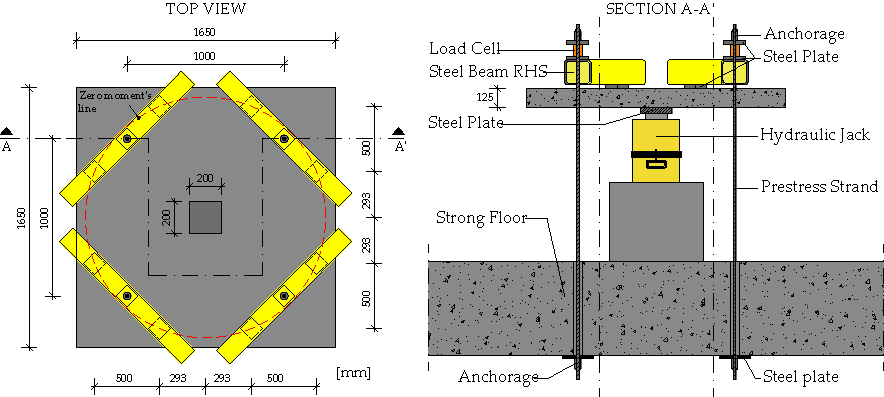
\includegraphics[width=\columnwidth]{Figures/i2015f1.pdf}\caption{Test setup\citep{inacio2015}.}\label{i2015f1}
    \end{figure}
    
\cite{qi2021} carried out concentrated load tests on eight similar flat slab specimens in three groups to study UHPC depth and area influence on flat slab punching shear behavior the application of which at full depth(\ref{q2021f1}) over the critical section area transformed the brittle punching shear failure mode into a ductile punching shear-flexure one while limited depth UHPC application over this area ended in brittle failure. 
\begin{figure}\centering
    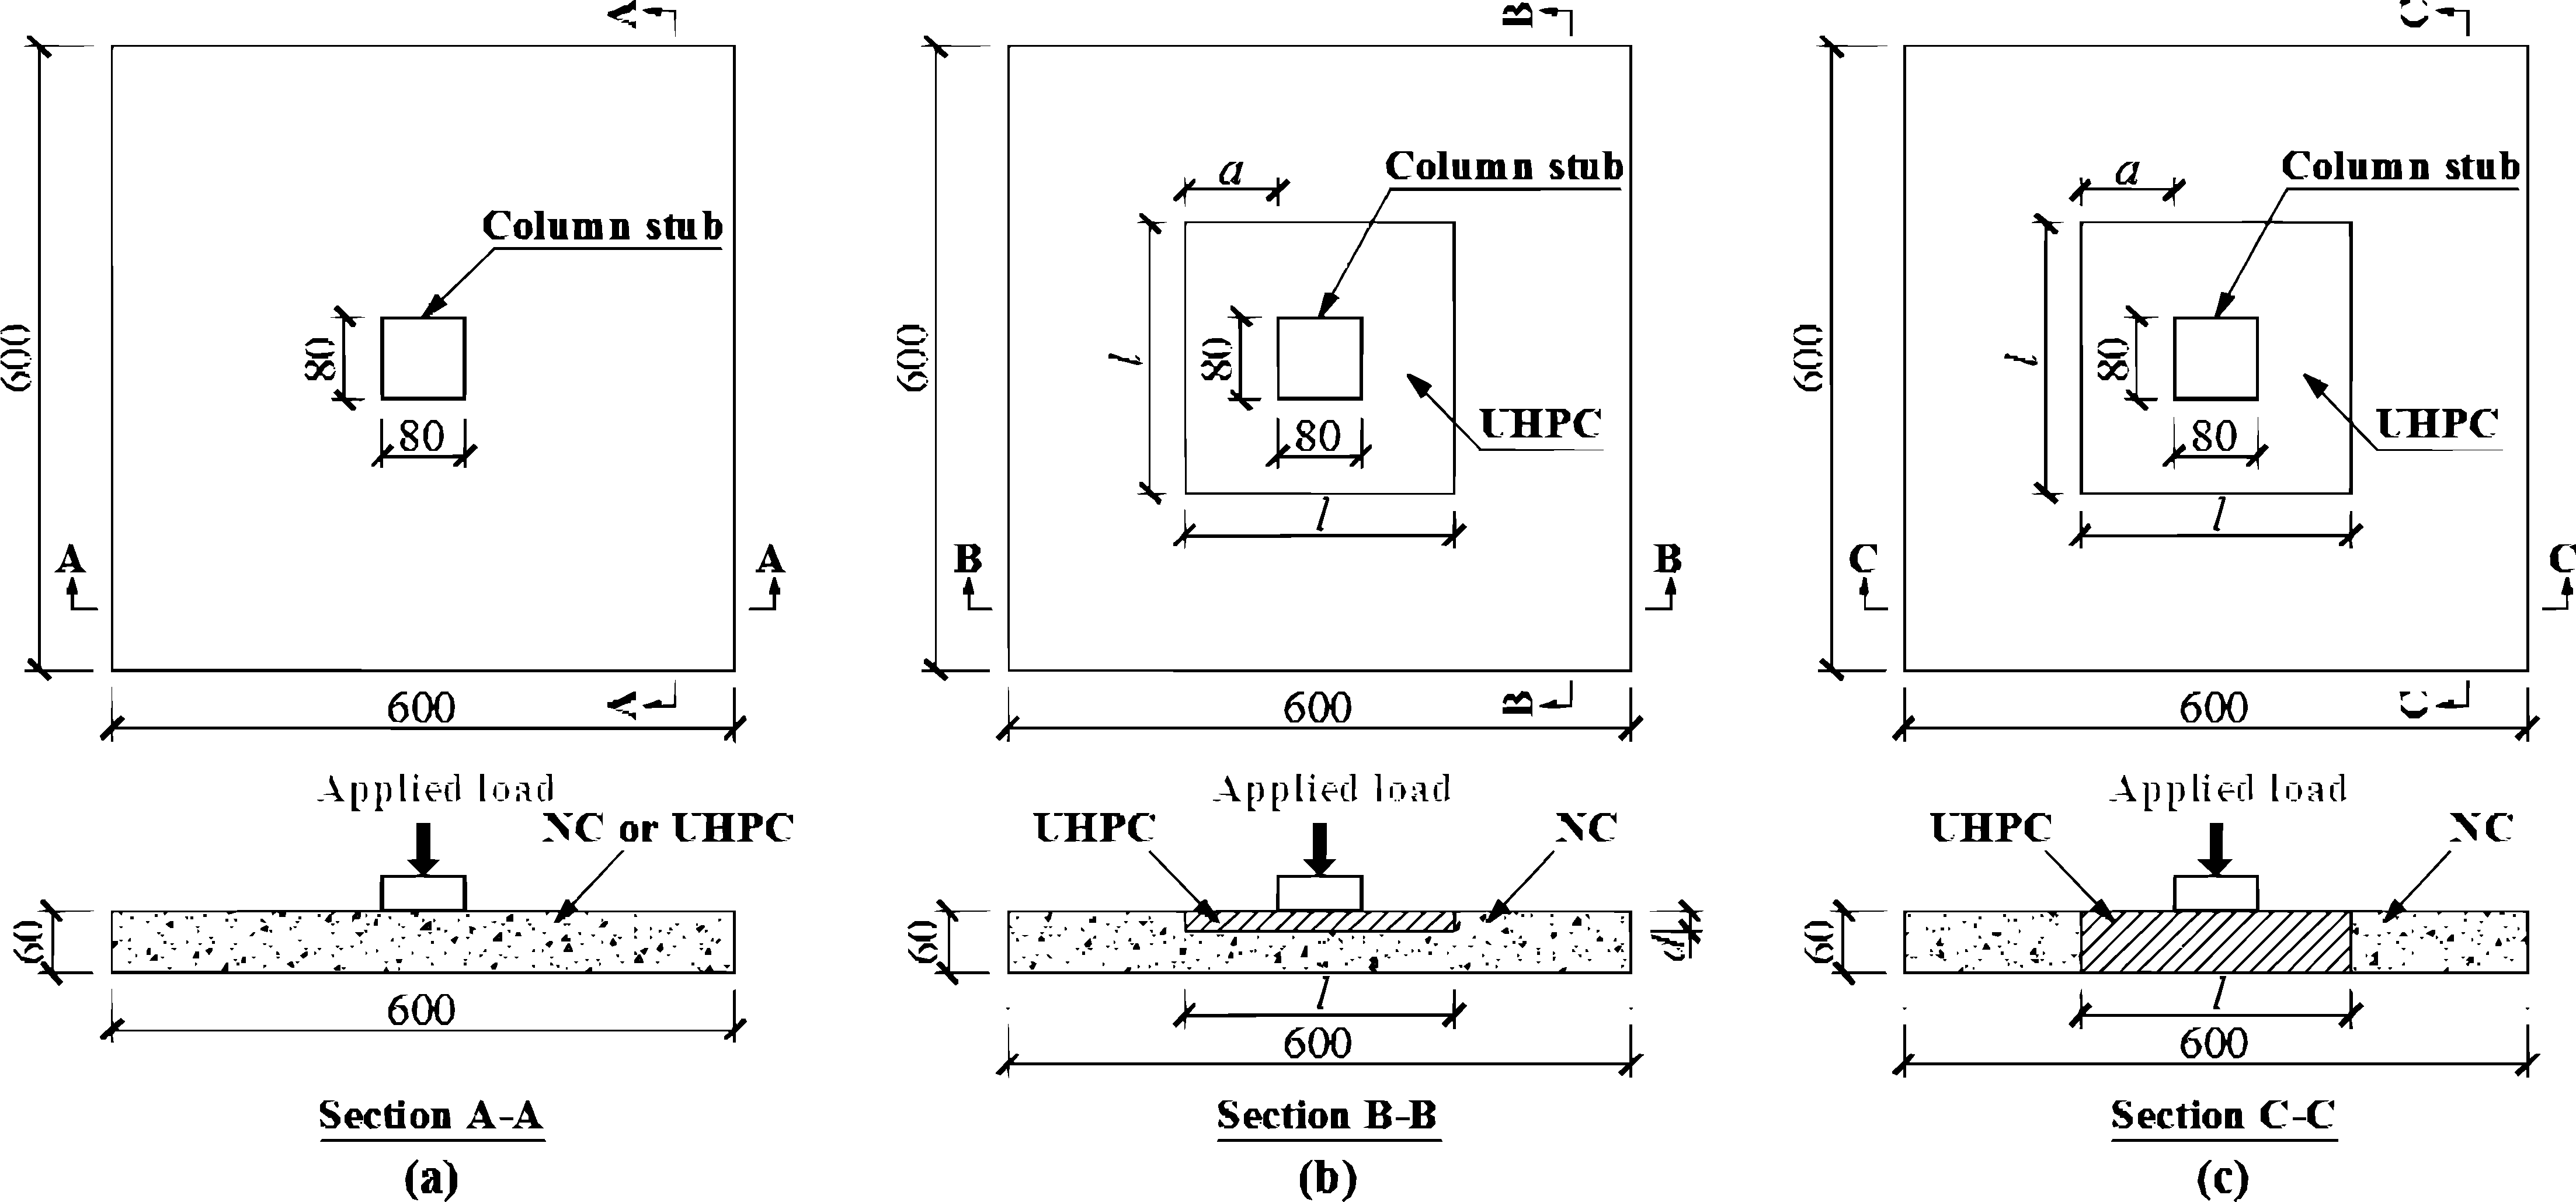
\includegraphics[width=\columnwidth]{Figures/q2021f1.pdf}\caption{Test setup\citep{qi2021}.}\label{q2021f1}
    \end{figure}
    
\cite{ramos2022} tried high-performance fiber reinforced concrete (HPFRC) application in slab-column connection vicinity as a substitute for shear reinforcement with four specimens under combined gravity and horizontal reversed cyclic loading in which connection drift capacity substantially improved compared to reference specimens and the HPFRC reinforced specimens performed better than specimens with HSC. \cite{ricker2017} carried out ten punching tests on slab-column connections with double-headed studs as shear reinforcement nine of which had fiber reinforced UHPC units in the slab-column connection compression zone(\ref{r2017f1}) that reached significantly higher failure loads compared to normal specimens. 
\begin{figure}\centering
    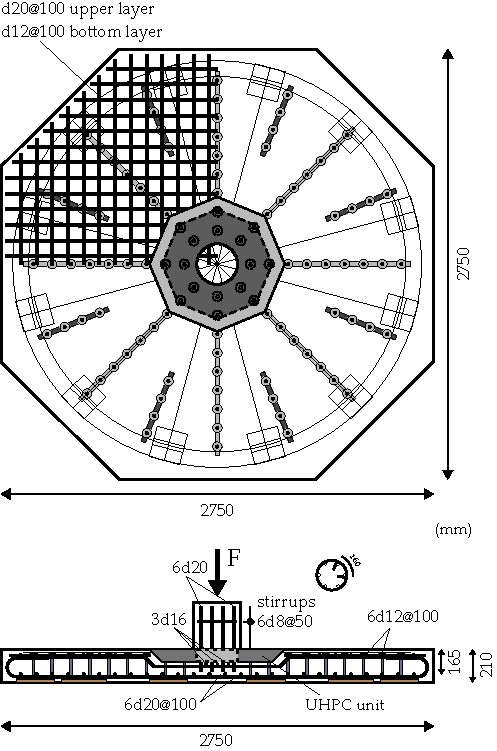
\includegraphics[width=\columnwidth]{Figures/r2017f1.pdf}\caption{Layout of flexural reinforcement and double-headed studs for test specimen DUHPC2\citep{ricker2017}.}\label{r2017f1}
    \end{figure}
    \begin{figure*}\centering
        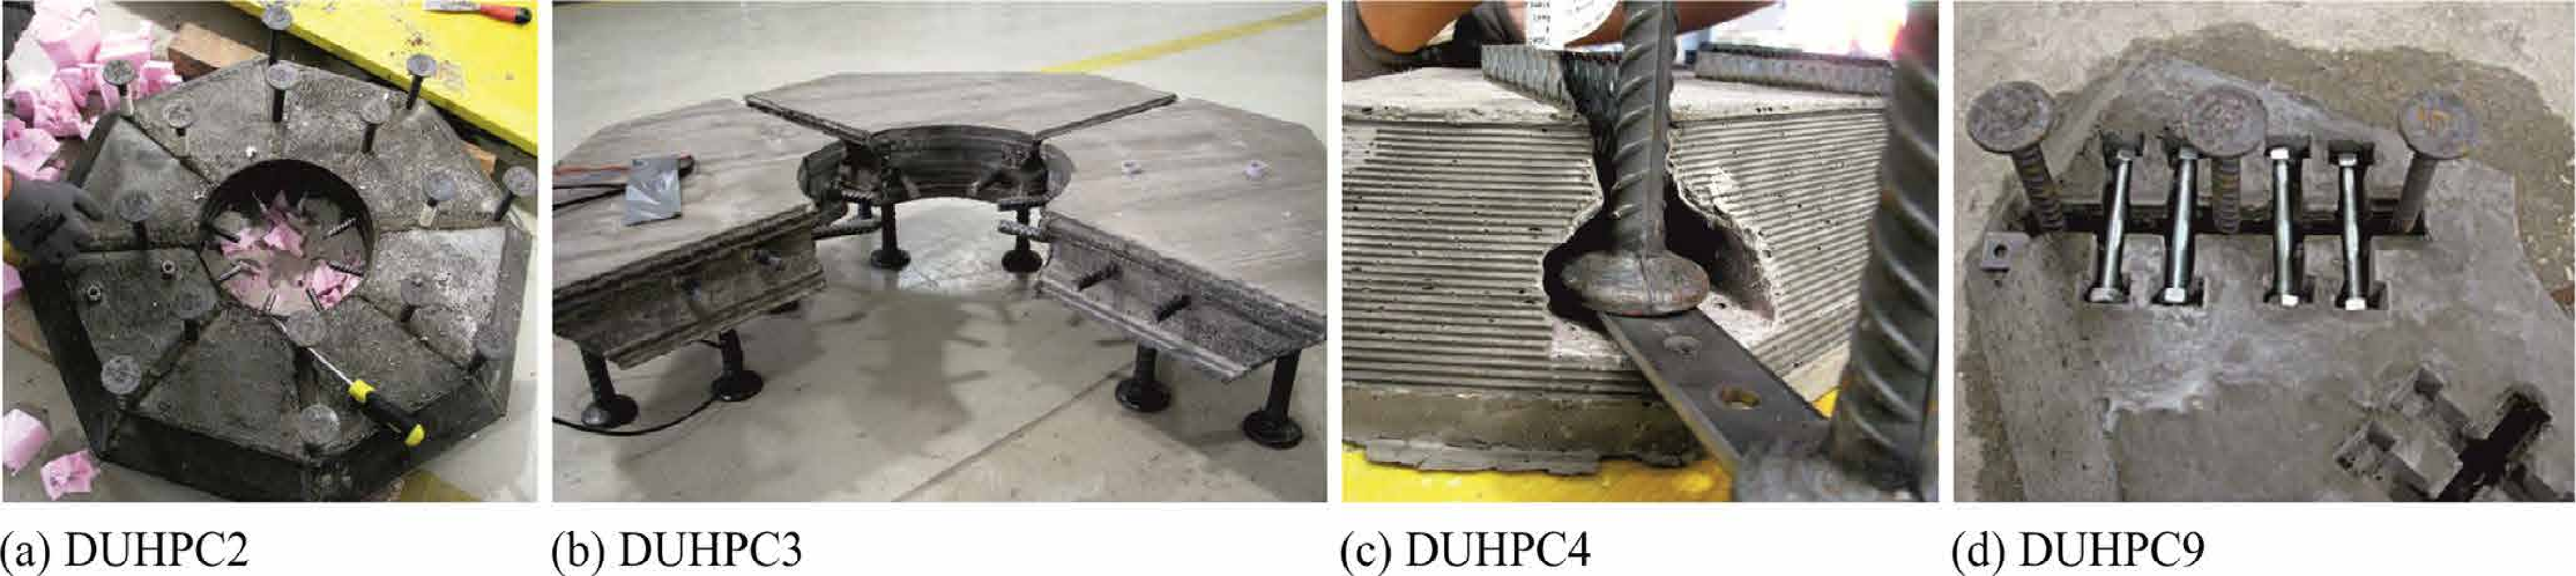
\includegraphics[width=\textwidth]{Figures/r2017f2.pdf}\caption{UHPC units\citep{ricker2017}.}\label{r2017f2}
        \end{figure*}
\cite{liu2023} improved punching shear performance of flat slab-column connections utilizing star-shaped steel plates (SSPs) in addition to engineering cementitious composites (ECC) replacing joint core concrete with five 1/2-scale connection specimens(\ref{l2023f3}).
    \begin{figure}\centering
        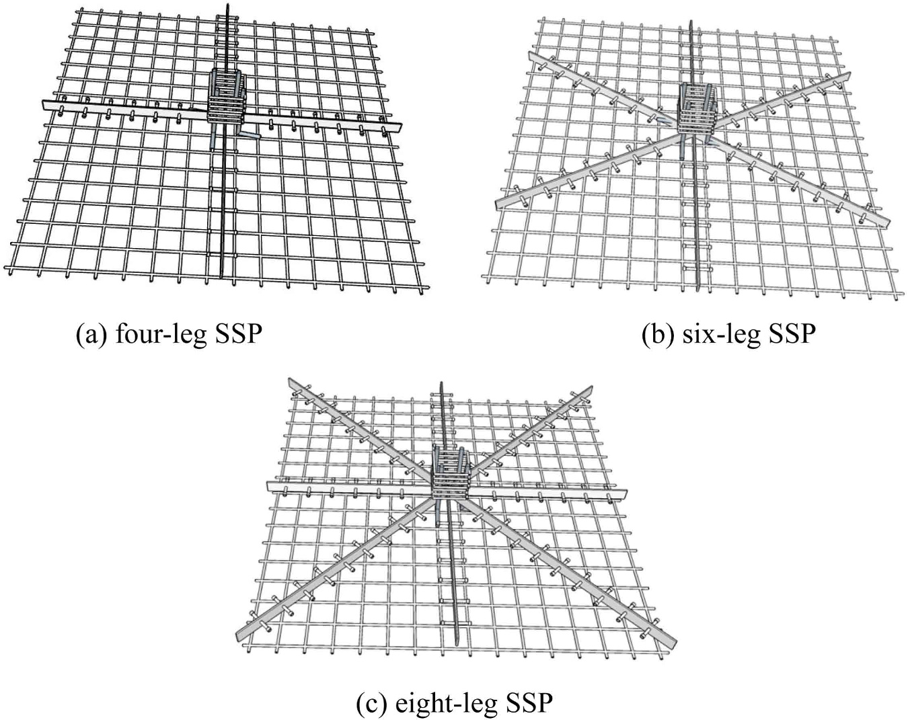
\includegraphics[width=\columnwidth]{Figures/l2023f3.png}\caption{SSP arrangement and configurations\citep{liu2023}.}\label{l2023f3}
        \end{figure}
Another concrete behavior improvement approach for slab-column joints has been introduced through the use of steel fiber additives in the concrete mix as studied by \cite{gouveia2018,gouveia2014,ABDELRAHMAN2018272,ju2015} that improves a plethora of structural characteristics in addition to punching shear strength including load bearing and flexural capacities along with structural stiffness and connection ductility. 

Carbon fiber reinforced polymer (CFRP) sheets were implemented by \cite{harajli2003} in a series of punching shear tests on slab-column connections as an additional reinforcement which led to significant improvements in flexural stiffness and strength along with higher connection shear capacity. CFRP and epoxy were successfully adopted by \cite{robertson2004} for damaged slab-column connection repair within a limited damage state. CFRP sheet efficiency in flat slab-column connection strengthening and rehabilitation/repair subjected to monotonic shear and unbalanced moment was nvestigated by \cite{polies2010} which despite loss of ductility showed promising restoration of connection ultimate load capacity and stiffness. \cite{esfahani2009} studied punching shear behavior of slab-column connections strengthened with CFRP sheets with variant width that resulted in way too conservative values based on \cite{ACI31814} suggestions. Punching shear behavior of CFRP grid reinforced concrete slabs was investigated by \cite{huang2020} while \cite{abdullah2013,saleh2019,akhundzada2019} investigated punching shear behavior of flat slab-column connection bonded with CFRP laminates. \cite{hamoda2019} carried out a numerical assessment of slab-column connection with extra CFRP bars. 
